\chapter{Object Definition and Reconstruction}
\label{sec:obj}
\textbf{LM fix} Does citations work here: \cite{trig-evtGen}?


\section{Jets}
\label{sec:obj-jets}
  \subsection{Hadronic cluster reconstruction}
  \subsection{Jet Reconstruction}
   anti-$k_T$
   \subsection{Jet calibration}
    (JES, JER, BJES) description
    
   \section{Identification of $b$-jets}
   \label{sec:obj-bjets}

   Hadronic jets, described in Section~\ref{sec:obj-jets}, can be further categorised into three seperate categories based on the flavour of the constituent quarks;
   \textit{b}-jets, \textit{c}-jets and light-flavoured jets, are defined as jets containing a \textit{b}-hadron, 
   a charmed-hadron or only light hadrons (only containing \textit{u},\textit{d} and \textit{s} quarks) respectively.
   \footnote{A more precise description of how this defined in a practice is given in Section~\ref{sec:obj-bjets_label}}
  
   The ability to identify $b$-jets is essential for a number of analyses within the ATLAS collaboration
   for example analyses that utilise the $t\bar{t}$ decay \cite{obj-ttbar} \footnote{Section~\ref{sec:trig-sys} contains a concrete example of this.}
   and the first direct evidence of the Higgs boson decaying to fermions \cite{obj-Hbb}.
   %In the former, as the top decays to a \textit{W}-boson and a \textit{b}-quark with a branching ratio close to 100\%, 
   %the application of $b$-tagging can be used increase purity, this is used in the study described in Section~\ref{sec:trig-sys}.
   %In the latter, the Higgs boson coupling is proportional to mass squared, hence the large mass of the
   %\textit{b}-quark means that $H\to b\bar{b}$ is the decay of the Higgs boson with the largest branching-ratio
   %which means that it is the best channel to make the first direct observation of the Higgs boson coupling to fermions.
   In the same sense, identification of $b$-jets is an essential part of the analysis being presented here;
   by selecting $b$-jets we increase our sensitivity to BSM models that decay to 1 or 2 $b$-jets in their final state.
    \textbf{Laurie Fix, reference where I explain why this is good, maybe Intro}.
   
   \subsection{Algorithm descriptions}

   The identification of $b$-jets, known as $b$-tagging,
   is performed by algorithms that utilise the long lifetimes (of the order ps) \textbf{Laurie Fix: Reference PDF?}
   of the heavy-hadrons that decay through the flavour changing weak interaction,
   A \textit{b}-jet decay chain  will typically contain two of these flavour changing interactions, 
   as at the quark level, the \textit{b}-quark contained in the jet will decay to a $c$-quark, which will then decay into a $u$ or $d$ quark.
   The long lifetimes of the heavy flavour hadrons means that they will decay a measurable distance from the 
   primary vertex, the point where the hard-scatter collision occurs, and hence the flavour can be inferred from the presence of particles 
   that originate from a point offset from the primary vertex.
   This is done using measurements from the tracks formed by the inner detector, in particular the precision silicon tracker,
   and the calorimter, which have been described in Section~\ref{sec:det-ID} and \ref{sec:det-calo}.
   
   There are three base $b$-tagging algorithms utilised to produce discriminating variables, which are described in the Sections~\ref{sec:obj-bjets_IP}~to~\ref{sec:obj-bjets_JF}.
   The variables are then combined in a multi-variate algorithm which is described in Section~\ref{sec:obj-bjets_MV2}.
   Figure~\ref{fig:obj_bjet_schem} shows a schematic illustrating how the tracks from the detector
   are used by the three $b$-tagging algorithms
   to identify the prescence of $B$-hadron in the jet.
   
   \begin{figure}[!htb]
     \begin{center}
       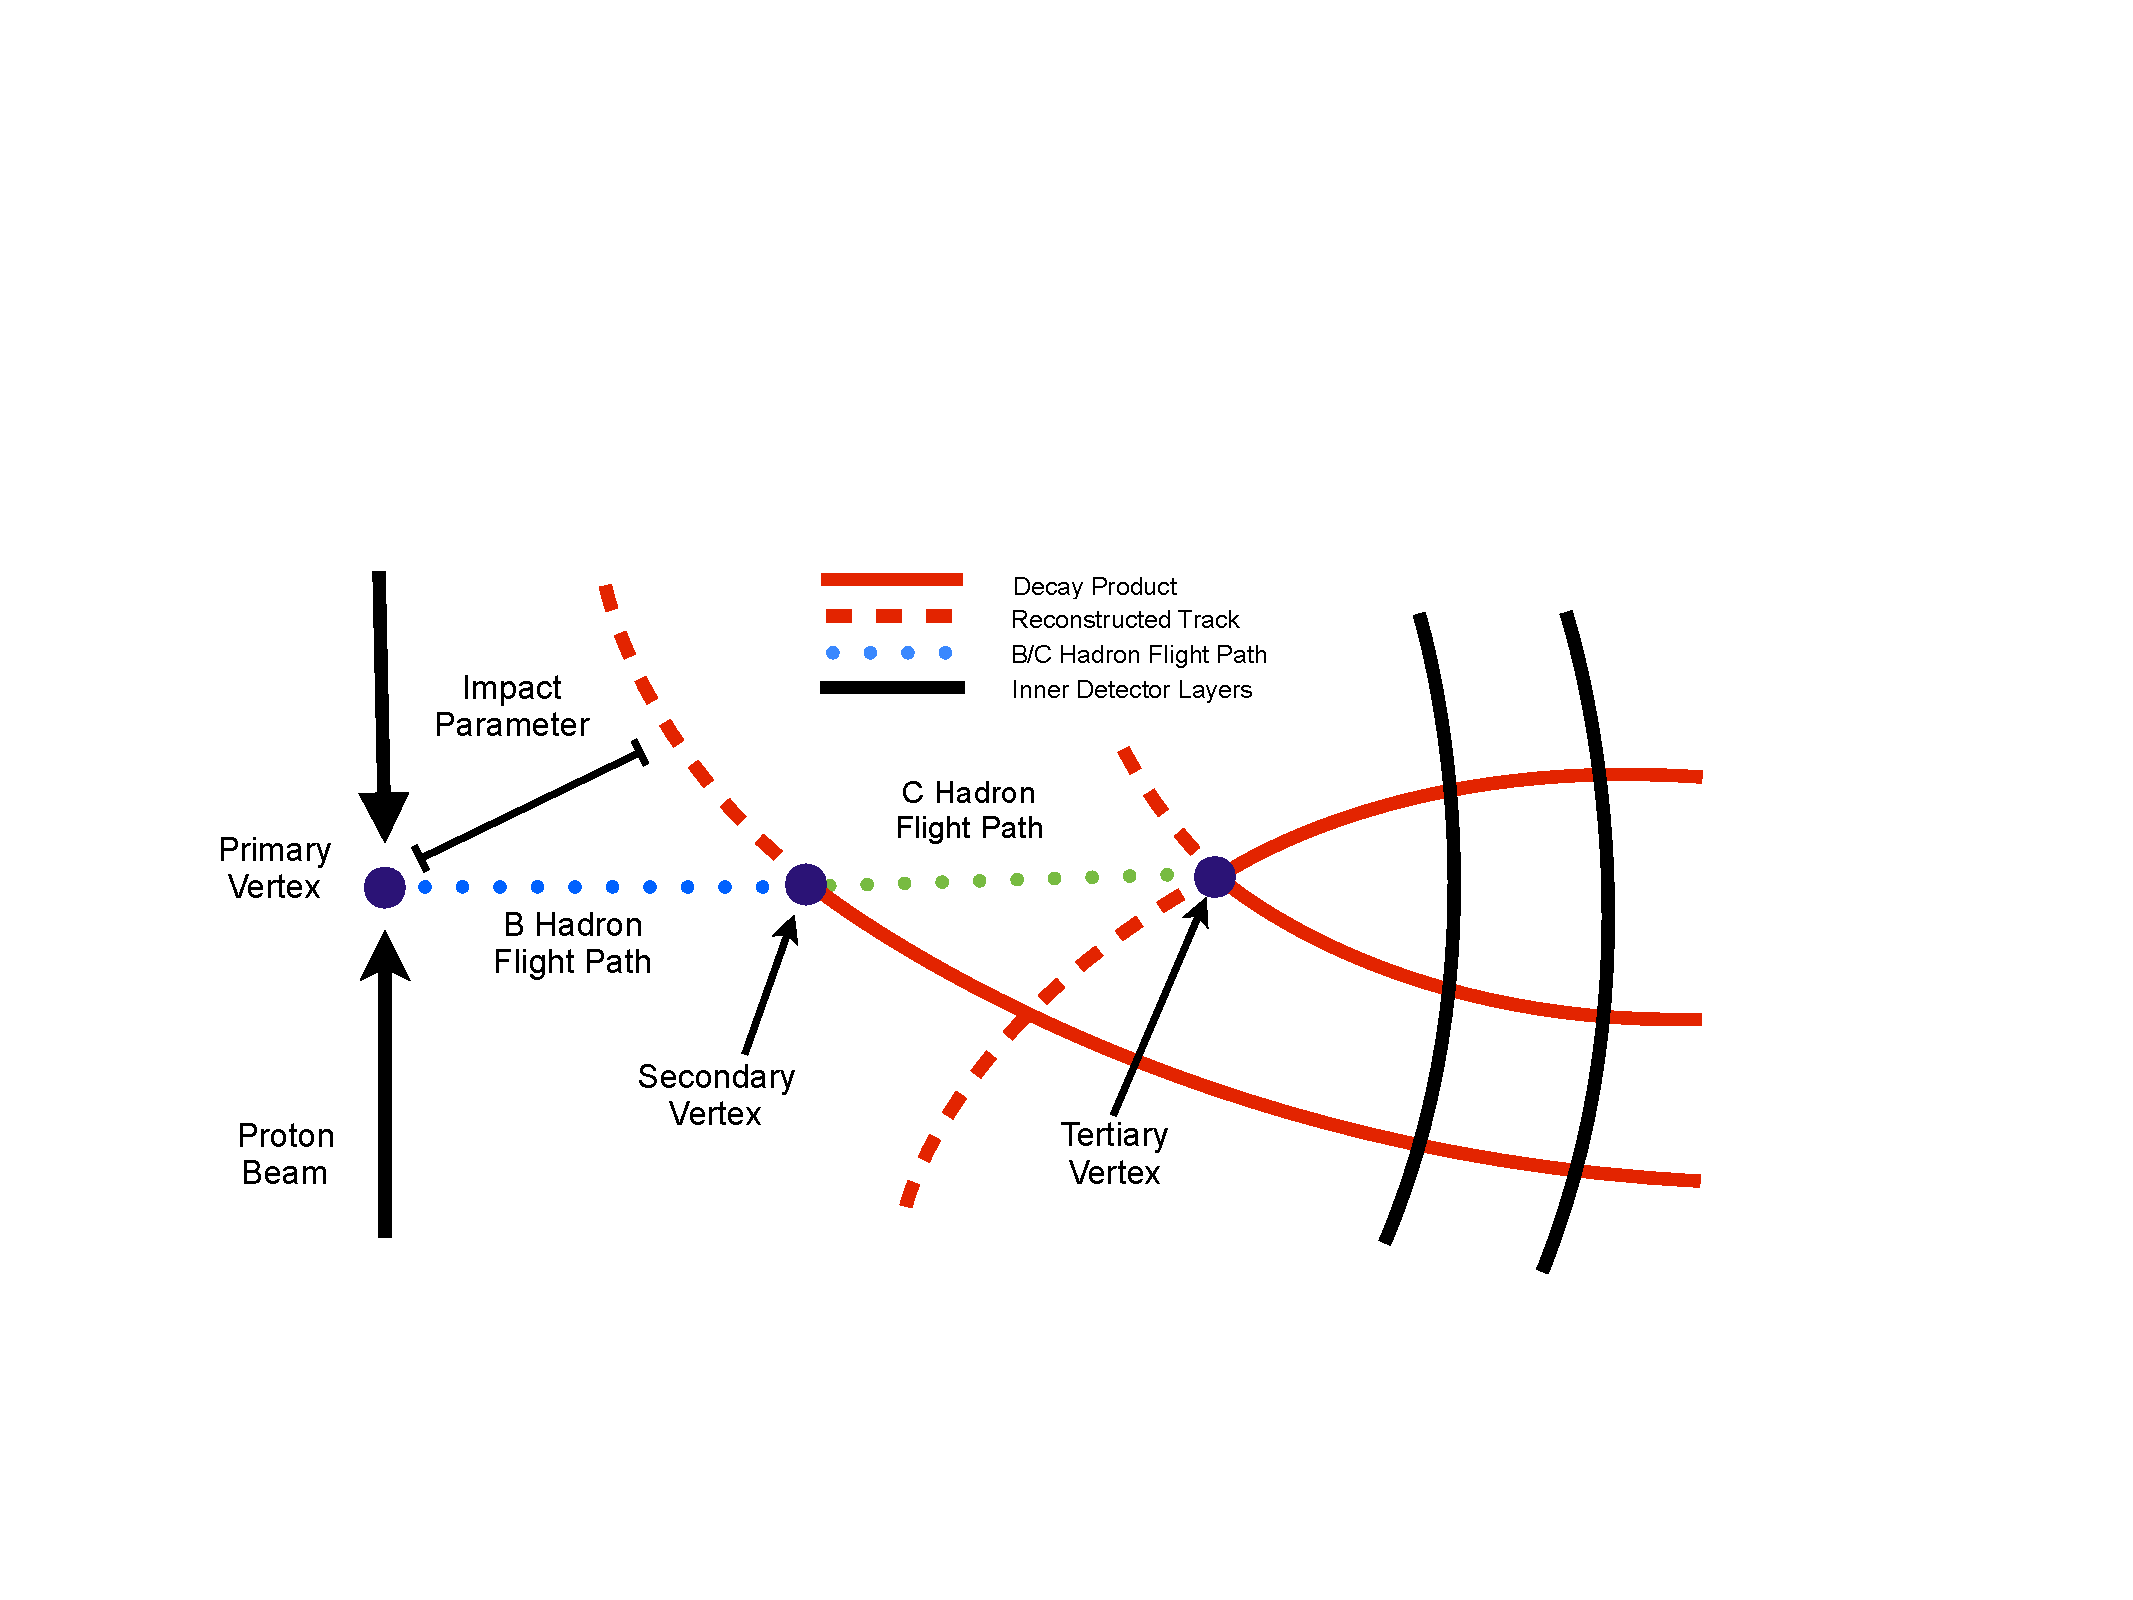
\includegraphics[width=0.9\textwidth]{figs/Objects/bjet_schem.pdf}
       \caption{A diagram to illustrate the key features of a $b$-jet that are utilised by the base $b$-tagging algorithms.}
       \label{fig:obj_bjet_schem}
     \end{center}
     \vspace{-0.5cm}
   \end{figure}

   \subsubsection{Impact parameter based}
   \label{sec:obj-bjets_IP}
 
   The IP3D algorithm is an impact parameter based flavour tagging tool. 
   A track corresponding to a particle coming from the offset decay vertex in a \textit{b}- or \textit{c}-jet is likely to have a large distance of 
   closest approach to the primary vertex, known as the impact parameter, meaning that the distribution of track impact parameter is different for each of the jet-flavours.
   In this algorithm, for all tracks associated to a jet, the impact parameter is calculated in both the transverse (perpendicular to beam-line)
   and longitudinal (parallel to beam-line) direction, which are referred to as $d_{0}$ and $z_{0}$.
   Then the IP3D algorithm calculates a likelihood of the jet having a specific flavour, 
   based on the distributions of the impact parameters ($d_{0}$, $z_{0}$), and the distributions of their significances 
   ($d_{0}/\sigma _{d0}$ and  $z_{0}/\sigma_{z0}$) of tracks inside the jet. 
   Another similar algorithm, IP2D, also calculates the jet flavour likelihood from just the transverse distributions, ($d_{0}$ and $d_{0}$ significance), which is more
   robust to pile-up, as tracks from pile-up jets are likely to have a large $z_{0}$ significance value.
   
   \subsubsection{Secondary vertex}
   \label{sec:obj-bjets_SV}

   
   The SV1 algorithm aims to reconstruct a secondary vertex of two or more intersecting tracks, corresponding to the decay of a heavy-flavour hadron. 
   Properties of the reconstructed secondary vertex that show flavour discrimination are, for example; the vertex 
   invariant mass and energy fraction (fraction of jet energy contained in the secondary vertex) which will be large for 
   \textit{b}-jets due to the heavy mass of the \textit{b}-hadron 
   \footnote{Mass of a B-meson $\sim$ 5 GeV and the mass of a D-meson $\sim$ 1.9 GeV, which are the most common heavy hadrons in a \textit{b}- and \textit{c}-jet respectively.}, 
   the distance in the transverse plane between the 
   primary vertex and the secondary vertex (2D flight path $L_{XY}$), which will be large for \textit{b}-jets due to the long lifetime of the \textit{b}-hadron,
   and the number of tracks at the secondary vertex, which will be large for well constructed secondary vertices, which are more likely in \textit{b}-jets.
   
   \subsubsection{Jet Fitter}
   \label{sec:obj-bjets_JF}

   The JetFitter algorithm (JF) attempts to reconstruct the full decay chain of the \textit{b}-hadron into a charmed-hadron and then into light-hadrons. 
   This is done by assuming that all vertices lie on a common \textit{b}-flight axis, and then constructing vertices from the intersection of
   one or more tracks and the flight axis.
   Reconstructed secondary and tertiary vertices correspond to the decays of the \textit{b}-hadron and charmed-hadron, as seen in Figure \ref{B-Tagging_Diagram}.
   Discriminating variables of JF, similarly to SV1, are vertex mass, energy fraction, number of vertices with two or more tracks and number of one track vertices.
   
   \subsubsection{Multi-variate}
   \label{sec:obj-bjets_MV2}

   
   The three base algorithms are combined in a boosted decision tree (BDT), which is a machine-learning technique for combining the many flavour-discriminating variables.
   As shown in Figure \ref{fig:obj-MV2_schem}, MV2 combines the likelihood output of IP3D and IP2D, with the discriminating variables of SV1 and JF discussed above.
   This is in contrast to the previous multivariate tagger used in Run-1, MV1, which inputted
   the likelihood of a jet having a certain flavour from each of the three base algorithms separately.
   For Run-2 the recommended \textit{b}-tagging tool is MV2c20 which has been trained on a sample containing 20\% charm, to give strong light- and \textit{c}-rejection rates.
 
   \begin{figure}[!htb]
     \begin{center}
       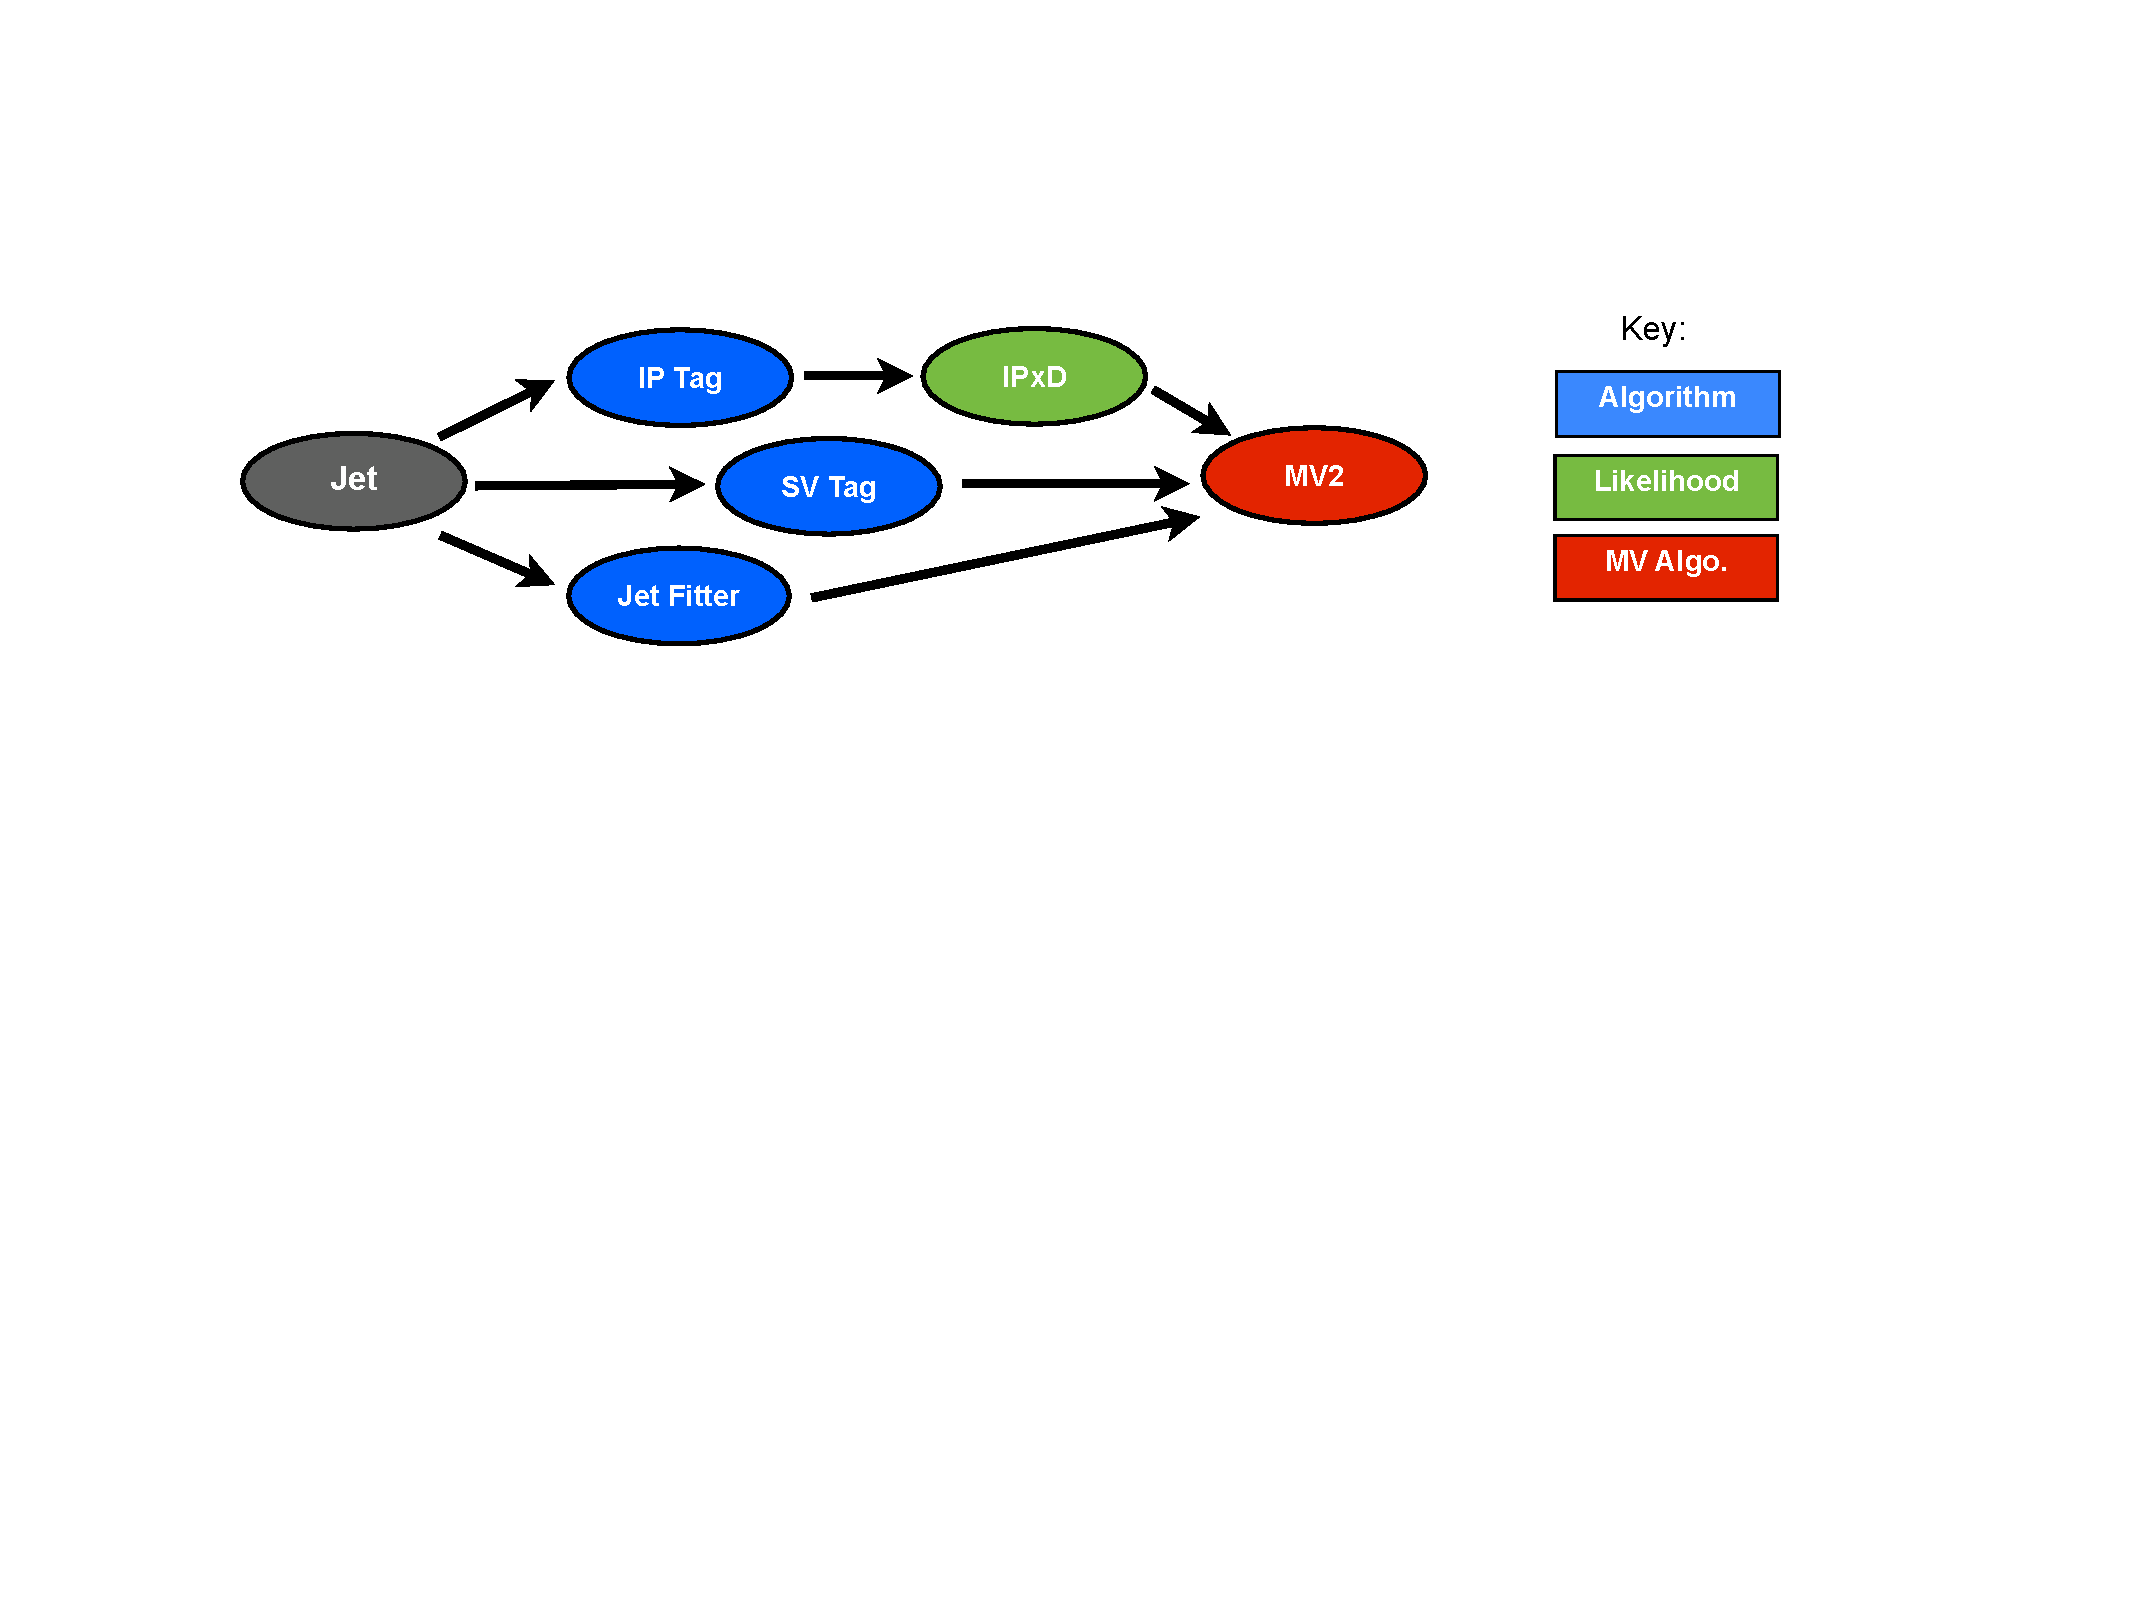
\includegraphics[width=1.0\textwidth]{figs/Objects/MV2_schem.pdf}
       \caption{A diagram to show the how the three base flavour tagging algorithms are combined in the MV2 algorithm.}
       \label{fig:obj-MV2_schem}
     \end{center}
     \vspace{-1cm}
   \end{figure}
   
   
   \subsection{Calibration/performance}
   \subsection{bTagging: Validation in Dijet Events}
    
  \section{Leptons}   
  \subsection{Electron}
  \label{sec:obj-electron}
  \subsection{Muon}
  \label{sec:obj-muon}
    
